\chapter{Knowledge Rapresentation}

\section{Knowledge Bases}

\subsection{Rappresentazioni Strutturate}

Durante la prima fase iniziale dell'IA ci si è concentrati sullo sviluppo di \fancyglitter{metodi generali} per la risoluzione di problemi\footnote{Tali metodi erano indipendenti da specifici domini.}. Successivamente, dalla seconda metà degli anni '60, si vollero abbandonare i domini astratti e semplificati per passare a problemi reali in cui era richiesta una \fancyglitter{conoscenza sul mondo in cui il sistema opera}.

\paragraph{Linguaggio e Operazioni:}

\begin{itemize}
  \item Vengono studiati i formalismi adatti a rappresentare le conoscenze necessarie. 
  \item Un sistema di conoscenza deve consistere di:
    \begin{itemize}
      \item Un \fancyglitter{linguaggio di rappresentazione}: un insieme di strutture sintattiche adatte a codificare le informazioni da rappresentare. 
      \item Un \fancyglitter{insieme di regole o di operazioni}: per manipolare il linguaggio.  
    \end{itemize}
  \item L'implementazione delle regole deve portare a \fancyglitter{inferenze desiderate} e le regole devono poter essere espresse come \fancyglitter{procedure}.
\end{itemize}

\paragraph{Strutturazione dell'informazione:}

\begin{itemize}
  \item Per rappresentare conoscenze è possibile utilizzare \fancyglitter{formule logiche} rappresentanti proposizioni indipendenti. 
  \begin{itemize}
    \item Con le formule logiche non è possibile collegare le varie formule, organizzandole in blocchi omogenei.
    \item La logica necessità di ulteriori meccanismi computazionali. 
  \end{itemize}
\item Esistono \fancyglitter{formalismi} per \fancyglitter{aggregare conoscenze elementari} in strutture più complesse. 
\item SI deve poter accedere alla struttura in cui le conoscenze relative all'oggetto in questione sono direttamente disponibili.
\end{itemize}

\dfn{Reti Semantiche}{
  Le reti semantiche sono un formalismo nato dai primi progetti di traduzione automatica. Hanno la caratteristica comune di utilizzare una struttura a grafo (rete) in cui i nodi rappresentano dei concetti e gli archi rappresentano relazioni tra concetti o proprietà dei concetti.
}

\cor{Grafi Relazionali}{
  I grafi relazionali sono le reti semantiche più semplici. Sono costituiti da grafi relazionali che permettono di descrivere le relazioni tra le diverse entità del grafo stesso.
}

\nt{Per esempio lo si può usare per descrivere uno stato nel mondo dei blocchi.}

\begin{figure}[h]
    \centering
    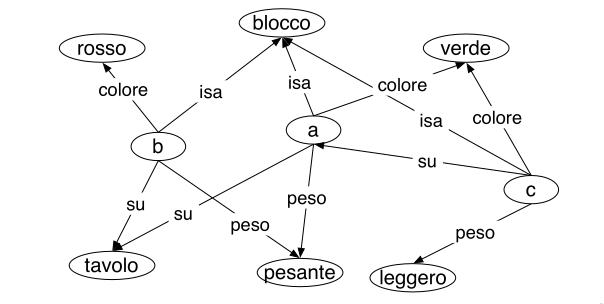
\includegraphics[scale=0.45]{02/mondo dei blocchi.png}
    \caption{Rappresentazione del mondo dei blocchi mediante grafo relazionale.}
\end{figure}

\clm{}{}{
  \begin{itemize}
    \item Il grafo è composto da diversi \fancyglitter{nodi} ognuno rappresentante un'entità. 
    \item Da ciascun nodo si dipartono \fancyglitter{archi} che lo collegano ad altri, sono \fancyglitter{etichettati} in modo da esplicitare la relazione che intercorre tra i nodi collegati. 
    \item Una relazione importante è \fancyglitter{isA}: il tipo di concetto che un nodo rappresenta.
  \end{itemize}
}

\paragraph{Espressività di un grafo relazionale:}

\begin{itemize}
  \item È implementato un \fancyglitter{sottoinsieme del calcolo dei predicati del primordine}: gli archi sono i predicati e i nodi sono i termini. 
  \item \fancyglitter{Limitazioni di efficacia espressiva:} i grafi rappresentano la congiunzione in maniera implicita. 
  \item È difficile rappresentare disgiunzione o implicazione. 
  \item Inoltre è complicato esprimere la quantificazione universale. 
  \item Le relazioni espresse dagli archi sono per loro natura binarie ma i predicati logici possono avere qualsiasi arietà.
  \item Una possibile soluzione è quella di tradurre tutte le relazioni in relazioni binarie:
    \begin{itemize}
      \item Accresce la granularità (e quindi l'espressività) e richiede l'introduzione di nodi per rappresentare oggetti e insiemi di oggetti e situazioni e azioni. 
      \item I predicati con arietà superiore a 2 esplodono in una serie di relazioni binarie: una che chiarisce il tipo di predicato, altre che esplicitano ruolo e funzione degli argomenti.
    \end{itemize}
\end{itemize}

\nt{Anche se una relazione ad alta granularità e una come formula del primordine formano un isomorfismo mettono in luce aspetti differenti.}

\cor{Reti Proposizionali}{
Le reti proposizionali sono reti semantiche i cui nodi possono rappresentare non solo entità semplici, ma intere proposizioni. 
}

\nt{Ammettendo la possibilità di avere nodi proposizionali si accresce l'espressività del linguaggio. Sono state proposte reti fortemente legate alla logica del primordine.}

\paragraph{La negazione:}

\begin{itemize}
  \item Può essere rappresentata mediante un arco che collega il risultato della negazione con la proposizione che viene negata. 
  \item Si possono rappresentare idee piuttosto articolate e distinguere tra: 
    \begin{itemize}
      \item \fancyglitter{Negazione di un'intera proposizione}. 
      \item \fancyglitter{Negazione di una proposizione incassata} all'interno di un'altra proposizione. 
    \end{itemize}
\end{itemize}

\begin{figure}[h]
    \centering
    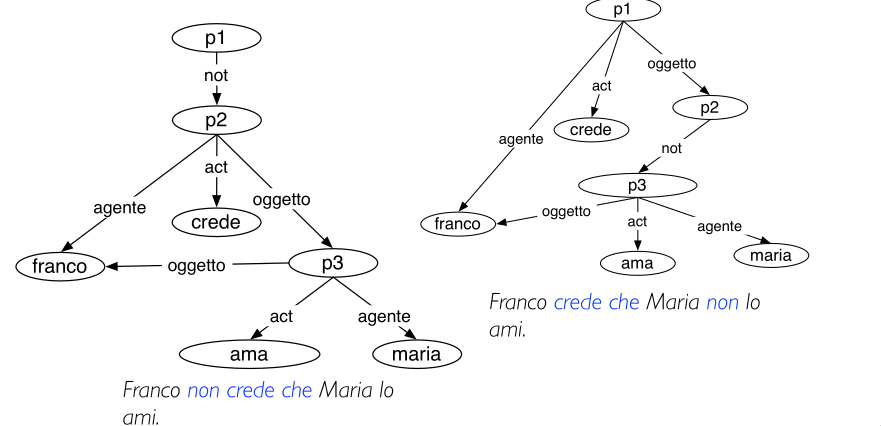
\includegraphics[scale=0.45]{02/prop.png}
    \caption{Introduzione della negazione.}
\end{figure}

\paragraph{Disgiunzione:}

\begin{itemize}
  \item Viene introdotta dopo la negazione. 
  \item Questo perché la congiunzione è implicita e si può rappresentare la disgiunzione in sua funzione mediante le \fancyglitter{leggi di De Morgan}.
\end{itemize}

\nt{La scelta di quale rete utilizzare va effettuata in base a leggibilità, flessibilità, efficienza, facilità di espressione, etc.}

\section{Rappresentazioni Gerarchiche}

Molte delle conoscenze sono organizzate in \fancyglitter{gerarchie}. Varie entità sono raggruppate in \fancyglitter{classi} che a loro volta sono raggruppate in \fancyglitter{sottoclassi}. Queste gerarchie non sono limitate a oggetti, ma si possono estendere ad azioni (e.g. camminare, marciare, etc.), eventi, stati, proprietà, etc. Per esempio, nelle reti semantiche se si vuole esprimere l'idea "gli elefanti sono mammiferi" è sufficiente un nodo per gli elefanti e uno per i mammiferi connessi da un arco etichettato isA. Così facendo si può fare inferenza, sfruttando proprietà delle relazioni (la relazione isA è transitiva). 

\subsection{Eredità delle Proprietà}

\dfn{Eredità delle Proprietà}{
Il meccanismo di eredità delle proprietà afferma che le proprietà asserite per un nodo valgono anche per i nodi che si trovano al livello inferiore della gerarchia.
}

\paragraph{Se la rete che rappresenta le diverse proprietà isA è un \fancyglitter{albero} è facile stabilire se un concetto $X$ gode della proprietà $p$:}

\begin{itemize}
  \item Per capire se $p(X)$ è vero basta considerare gli antenati di $X$ e vedere se qualcuno gode di $p$. 
  \item Questa ricerca è più efficiente dei processi di inferenza.
\end{itemize}

\paragraph{Vantaggi:}

\begin{itemize}
  \item \fancyglitter{Economia di rappresentazione:} invece di replicare una proprietà per tutti i nodi essa viene asserita solo al livello più alto in cui si applica. 
  \item \fancyglitter{Semplifica la manutenzione:} una modifica a una proprietà richide una sola operazione.
\end{itemize}

\paragraph{Trattamento delle eccezioni:}

\begin{itemize}
  \item Si può risolvere con un approccio procedurale. 
  \item Esempi: gli uccelli solitamente volano, ma alcuni no. I mammiferi partoriscono i figli, ma l'ornitorinco no.
\end{itemize}

\dfn{Validità per Default}{
Vengono rappresentate conoscenze che valgono fino a prova contraria. Le eccezioni vengono memorizzate in corrispondenza dei nodi a cui si riferiscono.
}

\nt{In questo caso si ottiene l'eccezione prima di raggiungere il nodo di Default.}

\dfn{Ereditarietà Multipla}{Nel caso una classe abbia più di una classe superordinata ($X$ isA $Y$, $X$ isA $Z$ con $Y \neg= Z$) la rete semantica passa da albero a grafo.}

\nt{Reti Semantiche 1, Java 0. \textit{If you know, you know}.}

\paragraph{Ammettendo l'ereditarietà multipla:}

\begin{itemize}
  \item Il tempo di ricerca passa da lineare a esponenziale, non esistono euristiche. 
  \item Nel caso di un \fancyglitter{conflitto di valori} non è possibile stabilire un criterio risolutivo che abbia carattere generale. 
  \item Diverse strategie: 
    \begin{itemize}
      \item Ricerca in profondità. 
      \item Ricerca in ampiezza.
    \end{itemize}
\end{itemize}

\paragraph{Problemi:}

\begin{itemize}
  \item [\textcolor{red}{\ding{55}}] Le tecniche di ricerca non permettono di giungere a risultati intuitivamente corretti. 
  \item [\textcolor{red}{\ding{55}}] I risultati sono inconsistenti. Esempio con Nixon Diamond: Nixon è sia pacifista che guerrafondaio.  
\end{itemize}

\dfn{Dissonanza Cognitiva}{
  Si può considerare la rete stessa come ambigua e in grado di esprimere più interpretazioni: ogni interpretazione è consistente con sé stessa, ma diventa inconsistente quando viene considerata con le altre.
}

\paragraph{Appartenenza e Inclusione:}

\begin{itemize}
  \item Non esiste una distinzione tra nodi che rappresentano individui e nodi che rappresentano classi o insiemi di individui. 
  \item Il legame isA viene usato per denotare sia l'\fancyglitter{appartenenza} (elemento in insieme) che l'\fancyglitter{inclusione} (insieme in insieme).
  \item Non si può distinguere tra proprietà vere per tutti gli individui di una classe e proprietà vere della classe in quanto tale. 
  \item È impossibile separare la semantica di una rete dal suo utilizzo.
\end{itemize}

\section{Frame}

Le persone utilizzano un insieme strutturato di conoscenze per interpretare le diverse situazioni che si trovano a dover affrontare. Quando ci si imbatte in una situazione si recupera una \fancyglitter{rappresentazione a carattere generale} che vienep poi raffinata e modificata.

\dfn{Frame}{
  Un frame è una struttura che rappresenta le conoscenze di carattere generale che un individuo ha riguardo situazioni, luoghi, oggetti, etc. Fornisce una cornice concettuale all'interno della quale vengono interpretati nuovi dati alla luce delle conoscenze derivate dall'esperienza precedente. 
}

\paragraph{Caratteristiche:}

\begin{itemize}
  \item Un sistema che usa i frame può \fancyglitter{formulare previsioni} e \fancyglitter{avere aspettative}. 
  \item Aiuta il processo di interpretazione di situazioni ambigue.  
  \item Vengolo facilitati il recupero di informazioni e i processi inferenziali.
\end{itemize}

\cor{Script}{
  Lo script è una struttura di conoscenza di alto livello che integra e organizza le frasi.
}

\subsection{I Frame per Rappresentare la Conoscenza}

\paragraph{Mancanza di una semantica formale:}

\begin{itemize}
  \item I frame rappresentano la conoscenza in maniera dichiarativa, ma senza una semantica formale. 
  \item Si presuppone l'esistenza di procedure in grado di utilizzare le informazioni contenute nei frame. 
\end{itemize}

\paragraph{Concetti nei frame:}

\begin{itemize}
  \item Livello di base: costituisce il modo naturale di categorizzare gli oggetti e le entità. 
  \item Livello superordinato/subordinato: rispettivamente generalizzazioni e specializzazioni di concetti di base.
  \item \fancyglitter{Prototipi:} membri tipici di una categoria. L'appartenenza viene categorizzata in maniera di maggiore o minore somiglianza rispetto ai prototipi (e.g. passero è migliore rappresentante di uccello rispetto ad airone che è migliore rispetto a struzzo).
\end{itemize}

\subsection{Strutture dei Frame}

\paragraph{Strutture gerarchiche:}
\begin{itemize}
  \item Gli elementi di un frame sono collegati da relazioni isA o \fancyglitter{ako} (a kind of) che consentono l'ereditarietà. 
  \item Le proprietà ad alto livello sono fisse, mentre ai livelli più bassi (sottoclassi o istanze individuali) possono essere specializzate.
\end{itemize}

\qs{}{Com'è fatto un frame?}

\begin{itemize}
  \item Ha un nome univoco. 
  \item Le caratteristiche sono rappresentate da un insieme di slot (caselle in cui viene inserito un determinato tipo di informazione). 
  \item Valori di default per gli slot. 
  \item Conflitti tra valori ereditati in caso di ereditarietà multipla. 
  \item Uno slot può essere una struttura complessa. 
  \item Procedure per rendere la computazione efficiente: 
    \begin{itemize}
      \item If needed: calcolo del valore di uno slot. 
      \item If added: solo quando si tenta di riempire uno slot.
    \end{itemize}
\end{itemize}

\section{Teorie del Significato}

\paragraph{Alcune teorie tipiche:}

\begin{itemize}
  \item Prototipi: come accennato in precedenza, si effettuano approssimazioni per rappresentare una categoria. 
\begin{figure}[h]
    \centering
    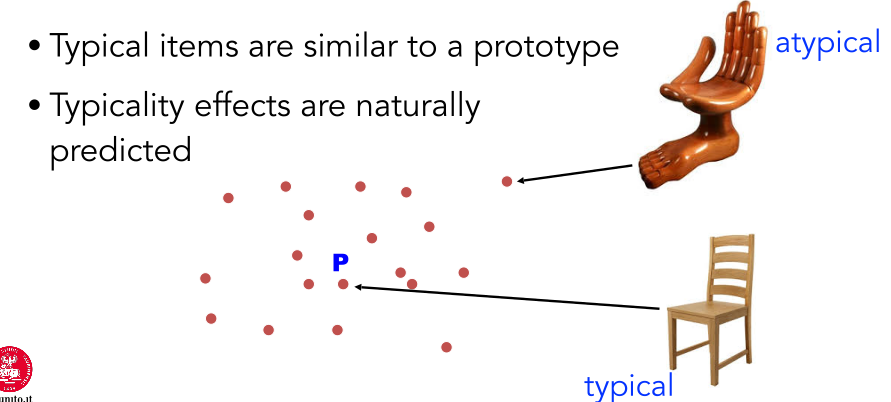
\includegraphics[scale=0.39]{02/prot.png}
    \caption{Teoria dei prototipi.}
\end{figure}

  \item Esempi: la rappresentazione mentale di un concetto è l'insieme di alcuni esempi di quella categoria.
    \begin{figure}[h]
    \centering
    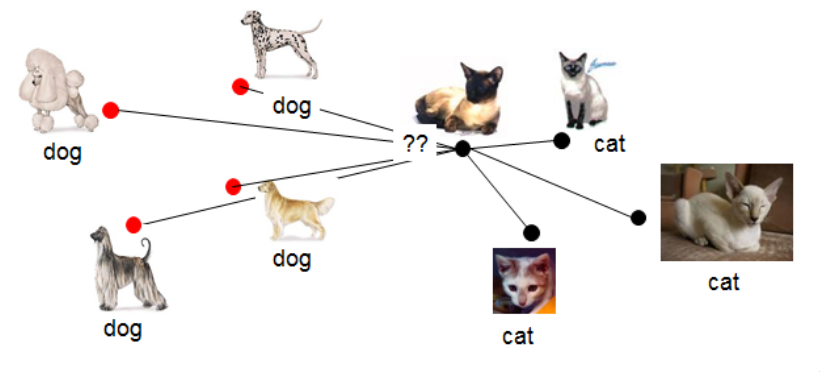
\includegraphics[scale=0.45]{02/exemplar.png}
    \caption{Teoria degli esempi.}
\end{figure}
  \item Teoria: i concetti sono parte della comprensione del significato, collegati ad altri concetti.
\end{itemize}

\nt{Quelle elencate qui sopra sono proprio tre teorie (probabilmente non avevano voglia di trovare nomi migliori).}

\paragraph{Approccio duale:}

\begin{itemize}
  \item \fancyglitter{Sistema 1} (implicito): categorizzazione non monotona, rappresentazione continua. 
  \item \fancyglitter{Sistema 2} (esplicito): categorizzazione monotona, rappresentazione dei dati proposizionale.
\end{itemize}

\subsection{Il Significato delle Parole}

\paragraph{Due problemi:}

\begin{itemize}
  \item Polisemia. 
  \item Semantica frasale.
\end{itemize}

\dfn{Contesto}{
  Il contesto è l'insieme degli elementi adiacenti a una parola. Può essere:

  \begin{itemize}
    \item Sintattico: elementi adiacenti a una parola dal punto di vista delle loro proprietà sintattiche. 
      \item Semantico: elementi adiacenti a una parola dal punto di vista delle loro proprietà semantiche.
      \item Linguistico. 
      \item Situazionale (pragmatico): richiede una conoscenza del mondo esterna alla lingua.
  \end{itemize}
}

\paragraph{Ambiguità e Polisemia:}

\begin{itemize}
  \item L'\fancyglitter{ambiguità} è la proprietà di una forma lessicale di avere più di un significato:
    \begin{itemize}
      \item \evidence{Contrastativa} (o omonimia): due significati contradditori. 
      \item \evidence{Complementare} (o polisemia): stessi significati in contesti diversi.
    \end{itemize}
  \item \fancyglitter{Principio di economicità linguistica:} si usano le stesse parole per esprimere più di un significato, per contenere le dimensioni del lessico, etc.
\end{itemize}

\nt{Solitamente i verbi tendono a essere più polisemici dei sostantivi.}

\dfn{Teoria Referenziale del Significato}{
  Le parole sono uno strumento attraverso il quale facciamo riferimento a ciò che esiste. Il significato delle parole consiste nella loro capacità di stabilire una relazione con elementi della realtà al di fuori della lingua.
}

\paragraph{Il riferimento può realizzarsi attraverso due procedimenti:}

\begin{itemize}
  \item \fancyglitter{Denotazione:} si indica la classe di elementi. 
  \item \fancyglitter{Designazione:} si indica un particolare elemento della classe. 
\end{itemize}

\paragraph{Interpretazioni:}

\begin{itemize}
  \item Ampia: ciascun elemento della lingua istituisce un riferimento con la realtà extralinguistica. 
  \item Restrittiva: distingue tra atto di riferimento e atto di predicazione.
\end{itemize}

\dfn{Teoria Mentalista}{
La teoria mentalista (o concettuale) arricchisce la teoria referenziale con l'ipotesi che il riferimento tra parole e realtà non sia diretto, ma mediato dall'immagine mentale dei concetti. Le parole non fanno riferimento diretto alla realtà extralinguistica, ma soltanto al modo in cui tale realtà è concettualizzata e categorizzata nella mente del parlante. 
}

\paragraph{Mediazione concettuale:}

\begin{itemize}
  \item Si può parlare non soltanto di entità esistenti o di eventi che accadono, ma anche di cose astratte, immaginarie o ipotetiche. 
  \item L'accento è sugli aspetti psicologici e sul legame tra concettualizzazione ed esperienza psico-percettiva.
\end{itemize}

\paragraph{Concetti e lessicalizzazione:}

\begin{itemize}
  \item I concetti cognitivi sono entità instabili: possono differire individualmente e culturalmente: 
    \begin{itemize}
      \item Appartengono alla struttura mentale. 
      \item Possono essere considerati come degli universali.
    \end{itemize}
  \item I concetti lessicalizzati sono più stabili: individualmente e socialmente condivisi: 
    \begin{itemize}
      \item Appartengono alla struttuea linguistica. 
      \item Variano da lingua a lingua.
    \end{itemize}
\end{itemize}

\dfn{Teoria Strutturale}{
  Il significato dei termini non è il suo riferirsi a un oggetto, ma nel valore che la parola assume in relazione alle altre parole presenti nella lingua che fanno parte dello stesso campo semantico.
}

\nt{Il valore semantico di un termine è il suo contenuo informativo.}

\dfn{Teoria Distribuzionale}{
  Il significato delle parole è determinato in larga misura dall'insieme di altre parole con cui queste co-occorrono. Questa teoria è ritornata di moda di recente grazie all'enorme disponibilità di corpora.
}

\cor{Metafora Geometrica del Significato}{
  I significati delle parole corrispondono a punti in uno spazio multidimensionale, in maniera tale che a punti vicini corrispondono parole con significato prossimo.
}
\nt{Questo è alla base delle rappresentazioni vettoriali e della cosine similarity.}

\subsection{Calcolo Sintagmatico del Significato}

\paragraph{Problemi fondamentali delle teorie del significato:}

\begin{itemize}
  \item Contestualità del significato. 
  \item Polisemia.
\end{itemize}

\dfn{Principio di Composizionalità del Significato}{
  Spiega come il significato degli enunciati si formi a partire dal significato degli elementi lessicali che li compongono.
}

\clm{}{}{
  In alcuni casi questo principio viene meno:
  \begin{itemize}
    \item Espressioni idiomatiche. 
    \item Usi metaforici. 
    \item Polisemia.
  \end{itemize}
}

\paragraph{Possibili approcci ai problemi:}

\begin{itemize}
  \item \fancyglitter{Enumerazione dei sensi:} i diversi sensi sono elencati nella parola, specificano i contesti in cui i diversi significati possono attivarsi. 
  \item \fancyglitter{Concezione dinamica:} le parole vengono concepite come entità permeabili e il significato di ciascuna interagisce con il significato delle parole adiacenti.
\end{itemize}

\paragraph{Principi di interazione semantica:}

\begin{itemize}
  \item Co-composizione: il significato di un verbo può essere determinato dai suo argomenti. Ciascun verbo ha una parte di base che non cambia, ma viene ridefinita e specializzata dal suo complemento. 
  \item Forzatura o conversione di tipo: un verbo in combinazione con un nome specifico lo spinge a significare determinate cose anche variandone il tipo semantico. 
  \item Legamento selettivo: l'aggettivo può selezionare una specifica porzione del significato del nome. 
\end{itemize}
